\documentclass[conference]{IEEEtran}
\IEEEoverridecommandlockouts
% The preceding line is only needed to identify funding in the first footnote. If that is unneeded, please comment it out.

\ifCLASSOPTIONcompsoc
  \usepackage[nocompress]{cite}
\else
  % normal IEEE
  \usepackage{cite}
\fi

\usepackage{caption}
\usepackage{graphicx, subfigure}
\usepackage{algorithm}
\usepackage[noend]{algorithmic}
\usepackage{textcomp}
\usepackage{multirow}
\usepackage{enumitem}
\usepackage{amsmath,amssymb,amsfonts}
\def\BibTeX{{\rm B\kern-.05em{\sc i\kern-.025em b}\kern-.08em
    T\kern-.1667em\lower.7ex\hbox{E}\kern-.125emX}}
\renewcommand{\algorithmicrequire}{ \textbf{Input:}} %Use Input in the format of Algorithm
\renewcommand{\algorithmicensure}{ \textbf{Output:}} %UseOutput in the format of Algorithm
%\renewcommand\thesection{\arabic{section}} 
%\renewcommand\thesubsection{\thesection.\Alph{subsection}} 

\begin{document}

\title{ Agile Adaptive Flow-Level Co-Sampling Strategy for SDN}

\author{He Cai$^{1}$, Jun Deng$^{1}$, Xiaofei Wang$^{1}$
\\
${^1}$Tianjin Key Laboratory of Advanced Networking, %School of Computer Science and Technology,\\
Tianjin University, Tianjin, China.
}


\maketitle

% As a general rule, do not put math, special symbols or citations
% in the abstract
\begin{abstract}
With the proliferation of Internet applications and the explosion of traffic, Fine-gaine's flow-level information acquisition provides basic support for network management, TE, security analysis, and Qos.In traffic sampling, due to the scale of the network, the analysis capcity of the Collector,and the highly random and dynamic network environment, there are a large number of flows cannot be captured. In this paper, we focus on maximizing sampling accuracy and sample effective ratio,proposing the Comprehensive Influence Maximization Collaborative Sampling(CIMCS) model.The model is modeled from sampling node selection, sampling time allocation, and cooperation between nodes to maximize the flow-level sampling accuracy and increase the sampling effective ratio. Based on the CIMCS, we propose three algorithms to solve the approximate optimal solution. We evaluated our strategy through a real large-scale topology, and the results show that it can effectively improve the sampling accuracy, especially in the mice-flow accuracy, and effectively improve the sampling efficiency.
\end{abstract}
%from the three dimensions of sampling node selection, time allocation and collaboration between nodes.
\IEEEpeerreviewmaketitle

\section{Introduction}

With the data traffic and network scale rapidly increaing, there exists huge demand for scalable network management. Flow-based measuresment is crucial to the network management. Accutate,timely and efficient flow-level statistics collection can provide assistance for security analysis,traffic engineering and intelligent routing. 

To solve the above problems, a agile, adaptive and cooperative sampling mechanism which can be applied to large-scale data center network is urgently needed. 

In this paper, we concentrate on how to address the above limitation and to achieve accurate and timely flow detection in the maximal value without modification to existing physical facility and extra burden to data center networks


\begin{figure}[!hhhhhhhhhht]
\centering
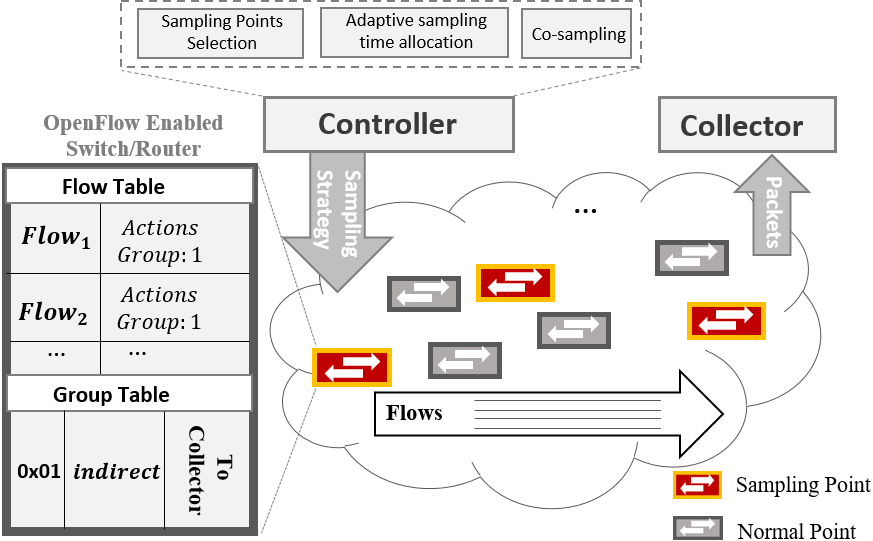
\includegraphics[width=8.5cm]{images/png_architecture.png}
\caption{Co-Sampling Architecture}
\label{Architecture}
\end{figure}

\section{Related Work}
Our main contributions are summarized as follows:
\begin{itemize}[leftmargin=*]
\setlength{\parindent}{0pt}

\item In the context of Flow-level Sampling, we focus on maximizing the sampling accuracy. From the three dimensions of  node selection,sampling node cooperation and time allocation, the CIMCS is constructed. We first explained the effect of cooperative sampling between nodes and packet repetition rate on sampling accuracy.
\item Based on the CIMCS optimization model, we split it into three sub-problems: sampling node election, Slot time allocation, and cooperation between nodes, and three heuristic algorithms are proposed to solve the approximate optimal solution of CIMCS.
\item We built the AAA platform and evaluated the performance of the algorithms using a real large-scale WAN topology. Finally, an application identification demo is implemented: App-Awareness.
\end{itemize}

\section{SYSTEM DESCRIPTION AND PROBLEM STATEMENT }

Figure \ref{Architecture} shows the framework of AAA. In the AAA mode, the SPS mode is used to collect the flow table entries of each group. All packets representing all the flows passing through the switch are copied to the unified group table entry to perform the actions defined by the group entry. When the controller controls the initialization of the group of entries, the action is initialized to point to the collector or discarded. Therefore, when the controller needs to control a switch to sample or stop sampling, it only needs to simply send a Group Mod message to the corresponding switch. When the action is Drop, the sampling is stopped. When it is directed to the exit of the collector, the sampling is started .This not only makes use of the pure OpenFlow protocol, but also controls it more precisely based on the controller's global. Assuming that the sampling period is $T$, through the adaptive coordination algorithm of AAA, the sampling points are selected and the sampling duration is allocated for them, and the sampling order is determined and the strategy is decentralized to the corresponding switch to make them cooperate sampling.

In large-scale networks, maximizing the sampling accuracy of Flow-level is a huge challenge to satisfy the low intrusiveness of the network and the maximum limitation of packet Collector (IDS e.g) analysis capability.Therefore, a highly agile and adaptive algorithm is needed to establish a sampling strategy for the real-time situation of the current network. When the network size is large, assuming the number of switches is $n$,$K$ ($K \le n$) nodes are generally selected as sampling nodes. And the value of $K$ is determined according to the actual situation.If the bandwidth of the collector is $C\, packets/T$, the total number of packets sampled by all nodes in a sampling period $T$ does not exceed $C$. Therefore, under the constraint $C$ and $K$, the reasons that affect the sampling accuracy include the selection of sampling nodes and the allocation of sampling time of each node. Another reason is the effective ratio of sampling.Packet repetition rate refers to different sampling nodes capture the same packet at almost the same time, called $E$, then the effective ratio is $1-E$. Collecting the same packet will not only occupy limited sampling resources and limit sampling accuracy, but also reduce the efficiency of the upper application (IDS e.g).Therefore, each sampling node must coordinate their own sampling time to reduce the overlapping sampling time as much as possible, thereby reducing the global packet repetition rate and improving the global sampling accuracy.

\subsection{CIMCS  Model}
In order to maximize the sampling accuracy of Flow-level, we build the model from three aspects: node selection, time allocation and cooperative strategy among nodes. We transform the maximum sampling accuracy problem to the maximum area coverage problem, as shown in Figure 2.In a period $T$, the flow set F in the whole network is just like an area depicted by a red solid line, then the set $F_i^ C$ of the flow detected by node $R_i$ is equivalent to the grey area, which is denoted as the direct value of the node.The red dotted area represents the potential value of the node, which is a new data flow that may be captured by the node in a $T$. These streams arrive only after the downward sampling strategy, so they are not perceived by the sampling algorithm.The overlap area of the grey area represents the same flow detected between the current nodes, as in $F_i ^ C \bigcap F_j ^ C$. The overlapping area of the red dotted line is the same new flow detected by each node.The sum of the direct value and the potential value represents the total value of nodes in a $T$. The larger the number of nodes detected, the greater the value of nodes. Therefore, the flow-level sampling problem can be directly converted to the area coverage maximization problem.If the sampling time of two nodes overlaps and $F^c_i \bigcap F^c_j \ne \varnothing $, this is considered to be flow overlap, then the number of overlapping streams should be subtracted when calculating the overall coverage area, which reflects the cooperative nature of the sampling nodes.Therefore, in order to maximize the sampling accuracy of flow, the more flow overlap in the system, the smaller the sampling time between nodes overlap.However, the red area of nodes is unknown when sampling strategy is formulated. Even by analyzing the flow arrival distribution model, we can not know the number of overlapping flows in the future of each node. Therefore, the potential value of nodes needs a separate or personal quantization.
\begin{figure}[!!!!!!!!!!!!!!hhhhhhhhhht]
\centering

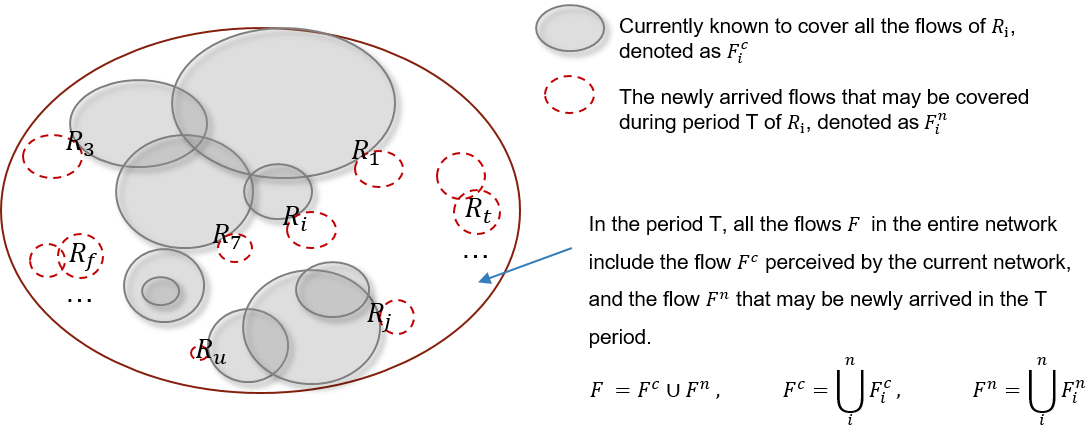
\includegraphics[width=8cm]{images/area_coverage.png}
\label{fig_1_area}

\caption{Area coverage problem}
\label{fig_1_model}
\end{figure}
We propose a quantitative approach based on influence, which transforms the direct value of nodes into direct influence and the potential value into potential influence. We evaluate the potential value of nodes from two dimensions:the power in a network[2] and the number of former flows.They all represent the potential influence of the node, which represents the potential value of the node, that is, the greater the potential influence, the greater the value that the node may create in a unit time.We used standardized mediation centrality [2] to measure the power of nodes in the network, and recorded the network impact of $R_i$ within a T as $S_i$.If the direct impact of $R_i$ is greater than $R_j$, but $S_j$ is higher than $S_i$, then even if the current flow deteced by $R_i$ is larger, the probability of the data flow passing through $R_j$ is greater later.The percentages of previous flows  reflects the activity of nodes throughout the network lifecycle, which we call historical influence. And we labeled the historical influence of $R_i$ within a T as $H_i $, $H_i = TF_i/TF$.So the potential influence of $R_i$ in a $T$ is the combination of $S_i$ and $H_i$.

Assuming that the arrival of packets of a flow $f_i$($i=1,2...,k$) obeys the Poisson distribution with ${\lambda_{i}}$. if any switch captures at least one packet from the same $f_i$, $f_i$ is considered to have been successfully captured. The probability of $f_i$ being captured in unit time $t$ is $P\{N_p^k (t) >0\}$.If you assign $t$ to the node $R_i$, the direct value of $R_i$ is $D_i$, which is show in (\ref{model_di}) .
\begin{equation}
D_i= \sum\limits_{{{f}_{k}}\in {{F}^{c}}}{P\left\{ N_{p}^{k}\left( t \right)>0 \right\}} /|F^c|
\label{model_di}
\end{equation}
Therefore, the acquisition rate of $R_i$is $D_i/|F^c|$, which we call direct influence.The quantification of direct influence is based on the flow betweenness centrality. Overall, $R_i$ has a combined effect of $\alpha \cdot {{D}_{i}}+\beta \cdot {{S}_{i}}+\gamma \cdot {{H}_{i}}$ over a $t$, and $\alpha +\beta +\gamma  = 1$.

We give CIMCS as (\ref{1}). 

\begin{equation}
\begin{split}
%\begin{gather}
\max \sum\limits_{i}^{n}{(\alpha \cdot {\delta ({{D}_{i}},\left| \widetilde{{{S}_{i}}} \right|)}+\frac{\left| \widetilde{{{S}_{i}}} \right|}{{T}/{t}\;}\cdot (\beta \cdot {{S}_{i}}+\gamma \cdot {{H}_{i}}))}  \\
-\frac{\alpha }{\left| {{F}^{c}} \right|}\cdot \sum\limits_{{{f}_{k}}\in {{F}^{c}}}{\sum\limits_{l=1}^{{T}/{t}\;}{\left( P\left\{ N_{p}^{k}\left( t \right)>0 \right\}\cdot \psi \left( {{f}_{k}},{{s}^{l}} \right) \right)}} \label{1}
%\end{gather}
\end{split}
\end{equation}

\begin{equation}
subject to: \sum\nolimits_i^n {f(\widetilde {{S_i}}) \le } K,f(\widetilde {{S_i}}) = \left\{ \begin{array}{l}
1,\left| {\widetilde {{S_i}}} \right| \ge 1\\
0,\left| {\widetilde {{S_i}}} \right| = 0
\end{array} \right.\label{2}
\end{equation}
\begin{equation}
\sum\nolimits_{i}^{n}{{{w}_{i}}\cdot \left| \widetilde{{{S}_{i}}} \right|\le C}\label{3}
\end{equation}

The goal of this model is to allocate the corresponding sampling time for each $R_i$ under the constraints of given $C$ and $K$, and to determine the sampling cooperation strategy among nodes, so as to maximize the influence of the system in the period $T$, and then maximize the flow-level sampling accuracy.Since time is continuous, let $t$ is the unit time, $t<=T$. And let $L = T/t$ represents the number of time slots ${{s}^{l}}($l=1,2...,L$)$ in the $T$.$\widetilde{{{S}_{i}}}$ represents the set of slots allocated to $R_i$.The larger the size $|\widetilde{{{S}_{i}}}|$ of slot set, the greater the combined influence of nodes.The relationship between the combined influence of nodes and $|\widetilde{{{S}_{i}}}|$ is given in (\ref{4}).
\begin{equation}
\delta \left( {{v_i},\left| {\widetilde {{S_i}}} \right|} \right) = \left\{ \begin{array}{l}
{v_i} \cdot \left| {\widetilde {{S_i}}} \right|,{\rm{    }}{v_i} \cdot \left| {\widetilde {{S_i}}} \right| < \left| {F_i^c} \right|\\
\left| {F_i^c} \right|{\rm{   }}\quad,\ {\rm{    ELSE}}
\end{array} \right.\label{4}
\end{equation}
When $ D_i\cdot |\widetilde{{{S}_{i}}}|>|F^c_i|$, it means that nodes can capture all the flows currently detected.Then its direct impact will not continue to increase with the increase of $|\widetilde{{{S}_{i}}}|$, but the potential impact will continue to increase. In addition, when a flow is collected by different nodes in the same slot, the actual number of flow in the whole system does not increase.Therefore, when the direct force of all nodes is accumulated in the left part of (\ref{1}), it may be calculated repeatedly.$U = \left\{ {{R_i},{f_k} \in F_i^c \wedge {s^l} \in \widetilde {{S_i}}} \right\}$ is a set of routers which are assigned the ${{s}^{l}}$ for detecing the $f_k$.When $|U|\ge 1$,the times $\psi ({{f}_{k}},{{s}^{l}})$ of $f_k$ counted repeatedly at ${{s}^{l}}$ is $|U|-1$(\ref{5}).
\begin{equation}
\psi \left( {{f_k},{s^l}} \right) = \left\{ \begin{array}{l}
\left| U \right| - 1,{\rm{    }}\left| U \right| \ge 1\\
{\rm{   }}0\quad \quad \; \; ,\, \left| U \right| = 0
\end{array} \right.\label{5}
\end{equation}
So the direct influence calculated repeatedly of whole network is ${\alpha \cdot P\{{{N}^{k}}(t)>0\}\cdot \psi ({{f}_{k}},{{s}^{l}})}/{{{F}^{c}}}\;$ via the $f_k$ at the ${{s}^{l}}$ ,in which $\alpha$ is a weight coefficient.In summary, the whole (\ref{1}) represents the summation of the comprehensive influence of all nodes, and then subtracts the direct influence calculated repeatedly of all nodes to obtain the total influence of the system. Just like area coverage, the area of overlapping parts is calculated many times without increasing the actual area coverage.

(\ref{2}) (\ref{3}) describes the constraints that the CIMCS model should satisfy. The number of sampling nodes $f(\widetilde{{{S}_{i}}})<= K$, and the number of sampling packets $w_i \cdot |\widetilde{{{S}_{i}}}|<=C$ sampled in period $T$. In (\ref{3}), $w_i$ is the price of $R_i$ in unit time $t$. If the current rate of $R_i$ is $w_i\, packets/T$, (\ref{6}) describes the calculation process of $w_i$, and $w_i*[(\beta \cdot {S_i}+ \gamma \cdot {H_i}/\alpha \cdot {D_i}]$ represents an estimate of the possible arrival rate of the node. The cost of the new flow that the nodes may arrive in the $T$ is not negligible. We use the ratio of influence to estimate the equal ratio.
\begin{equation}
{{w}_{i}}=\frac{t}{T}\cdot [{{\nu }_{i}}\cdot (1+\frac{\beta \cdot {{S}_{i}}+\gamma \cdot {{H}_{i}}}{\alpha \cdot {{D}_{i}}})]\label{6}
\end{equation}

We explained the quantization process of the CIMCS model and illustrated it as $Fig.2$.The goal of the CIMCS model is to allocate reasonable $|\widetilde{{{S}_{i}}}|$ sets for all $R_i$ under constraint conditions.As $Fig2$ shows, when the system gets the optimal solution of $S ^ 1. S ^ n $, it not only reflects the optimal node selection, the optimal time allocation, but also reflects the optimal slot order, which is determined by the cooperation strategy between nodes. At the same time, each node actually avoid overlapping on the same slot as much as possible, so that the effective ratio of the system is improved.

 

\begin{figure}[!!!!!!!!!!!!!!hhhhhhhhhht]
\centering

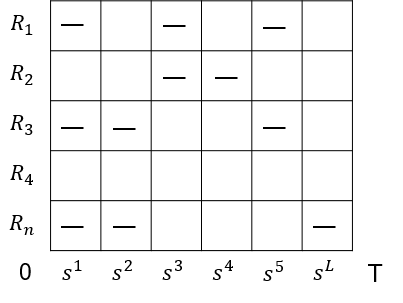
\includegraphics[width=8.5cm]{images/slot_num_order.png}
\label{fig_1_slot}

\caption{Overview of model}
\label{fig_1_model}
\end{figure}



\section{Optimal}
Since the above model is complicated, we divide it into three sub-problems: K node selection, Slot allocation, and collaborative sampling optimization. The solution to each sub-question will be the input to the next sub-question. Through three steps, the approximate optimal solution of the total problem is obtained.In this section, we detail each sub-question and propose the corresponding algorithms.
\subsection{Iterative comprehensive influence-based $Top-K$ node selection based on flow privatization} 
In the selection of K sampling points, we only focus how to use the static properties of the nodes to quantify their comprehensive influence, which is independent of time allocation. In (\ref{1}), when the number of slots and the cooperative relationship between nodes (slots order) are not considered, the optimization formula can be expressed as (\ref{maxk}) and the constraint is (\ref{maxkc});The goal of the optimization model \ref{maxk} is to select K sampling nodes without considering the influence of time on the comprehensive influence of the nodes, so as to maximize the comprehensive influence of the system.Similar to the CIMCS model, the former part sums the comprehensive influence of the selected nodes, and the latter part subtracts the influence part of the repeated calculations.
\begin{equation}
\max [\sum_{i=1}^n (\alpha \cdot {D_{i}} + \beta \cdot {S_{i}} + \gamma \cdot {H_{i}}) \cdot \varphi{(i)} - \alpha \cdot\sum_{f_k \in F^c} \widehat{\psi}{(f_k)}]
\label{maxk}
\end{equation}
\begin{equation}
subject to:\sum_{i=1}^{n} \varphi(i) = K
\label{maxkc}
\end{equation}
In(\ref{maxk}), $D_i=|F^c_i|/|F^c|$,and $\varphi(i)$ is 0 means that $R_i$ is not selected, 1 means $R_i$ is selected;$\widehat{U} = \{R_i,f_k \in F^c_i \wedge \varphi(i) = 1\}$ indicates how many selected nodes cover $f_k$,so the(\ref{maxkr}) indicates how many selected nodes are repeatedly calculated $f_k$ as their direct influence.Therefore, the subtracted part expresses that any flow will only be calculated once as a direct influence,in other words, any flow will only be calculated as direct influence by only one of the selected nodes, the flow is privatized by a selected node during the selection process.
\begin{equation}
\widehat{\psi} \left( {{f_k}} \right) = \left\{ \begin{array}{l}
\left| \widehat{U} \right| - 1,{\rm{    }}\left| \widehat{U} \right| \ge 1\\
{\rm{   }}0\quad \quad \; \; ,\, \left| \widehat{U} \right| = 0
\end{array} \right.
\label{maxkr}
\end{equation}
Therefore, it is possible to iteratively calculate the top $K$ nodes with the most comprehensive influence, the highest comprehensive influence in each round will be selected, and privatize all the flows it covers (but not including the flows privatized by other selected nodes in the previous);That is, for the direct influence of the candidate $R_i$ in the $k$ round, use the flow set $\widetilde{F}^{cs}_i$ to calculate the direct influence; Let $F_k^{cs}$ denote the set of flows privatized by the selected node in the $k_{th}$ round, so $\widetilde{F}^{cs}_i = F_i^c- \bigcup_{m=1}^{k-1}F_m^{cs}$,and the subtracted portion indicates that it has been privatized by the selected node of the previous k-1 round;If $R_i$ is selected in this round, the flows in $\widetilde{F}^{cs}_i$ is $R_i$ exclusive,then $\widetilde{F}^{cs}_i$ written as $F^{cs}_k$,$R_i$ is written as $R^s_k$; In the $k+1$ round selection, even if the other candidate nodes cover these flows, these flows have been privatized by the $R_i$, will not bring value to these candidate nodes in the $k+1$ round. The K-round selection is carried out, and the nodes with the highest comprehensive influence are selected in each round,through the process of privatizing the flows with the most influential nodes in each round, any two selected nodes are: $F^{cs}_i \bigcap F^{cs}_j = \varnothing$, and the comprehensive influence of each node is the highest in the corresponding round, so the K selected nodes guarantee (\ref{maxk}) to be maximized under the constraint (\ref{maxkc}). so the $K$ nodes are the optimal solutions.$D_i^k$ indicates the direct influence of the candidate node $R_i$ in the $k-th$ round selection, which $D_i^k = |\widetilde{F}^{cs}_i|/{\left| F^c \right|}$. (\ref{maxki}) describes the iterative calculation formula for the comprehensive influence of the candidate nodes for each round of selection.
\begin{equation}
I_{i}^{k}=\alpha \cdot D_{i}^{k}+\beta \cdot {{S}_{i}}+\gamma \cdot {{H}_{i}}
\label{maxki}
\end{equation}
Algorithm 1 gives the solution process, and Fig3 also shows the change process of direct influence in each round of elections.Finally, the K node set $R^s$ and the $F^{cs}$ set corresponding to each node can be obtained.The time complexity of the algorithm is $O(K*|R|)$.


\begin{algorithm}[h]
\caption{Sampling Point Selection}
\begin{algorithmic}[1]

\STATE define $R^s=\varnothing$  //  The Set of Selected Routers

\FOR{$k=1$; $k < K$; $k++$ }

\FOR{each $R_i \in R-R^s$}
\IF{$I_i^k > max$}
\STATE $max = I_i^k$
\STATE $R^s_k = R_i$
\ENDIF
\ENDFOR
\STATE put $R^s_k$ into $R^s$
\STATE $F_K^{cs} = F_i^c- \bigcup_{m=1}^{k-1}F_m^{cs}$ 
\ENDFOR

\RETURN $R^s$
\label{code:recentEnd}
\end{algorithmic}
\end{algorithm}


 


\subsection{Non-starved influence change-aware priority polling slot allocation}

After the node is selected, the number of Slots needs to be allocated to these nodes when the constraint (10) is satisfied and the Slot sequence between nodes is not considered.The optimization model of the subproblem is the (\ref{dasd}), which is still judged by the formula (3).The goal of the model is to maximize system value under the given $R^s$ and constraints (10). The reason why the model does not need to consider the influence of overlapping flows between nodes on the total influence of the system is that we use the privatized flows set of each node $F^{cs}$ to quantify the direct influence of each node,and arbitrarily $F^{cs}_i \bigcap F^{cs}_j = \varnothing$, so the direct influence in the node $R_i$ in unit time t is (\ref{newDI}).
\begin{equation}
{D}_i=\frac{\sum_{f_k \in F^{cs}_i} P\{N_p^k(t)> 0\}}{|F^c|} 
\label{newDI}
\end{equation}
For the cost $w_i$ of the node in unit time t, still uses $F_i^c$ to calculate. This is because we only logically eliminate the overlapping flows between nodes, but there is still no change in the overall rate of the underlying nodes.$CNT[1..K]$ represents the number of slots for each node.
\begin{equation}
\max [ \alpha \cdot \delta(D_i,CNT[i]) + \frac{CNT[i]}{L}(\beta \cdot S_i + \gamma \cdot H_i)  ]
\label{dasd}
\end{equation}
In the sub-problem optimization model, the comprehensive influence of the nodes increases with the increase of the number of Slots. When the situation of ELSE in formula (3) is satisfied, another growth trend will be presented,and he trend depends on $S_i$ and $H_i$. We have described the reasons in the construction of the CIMCS model.That is to say, the value generated by a single Slot is related to the number of Slots, not independent, so it is not possible to solve the optimal solution with multiple backpacks.

We give a simple and efficient allocation algorithm to achieve: the simple influence of the node's comprehensive influence per unit time t from high to low polling allocation, so that the current high-influence nodes preferentially allocate Slot.After each round of allocation, if a node satisfies the ELSE condition of formula (3), the comprehensive influence of the node in unit time t is $\beta \cdot S_i + \cdot H_i$,which does not satisfy the formula ( 3) For ELSE condition, continue to use the comprehensive influence of the three weighted sums.The algorithm stops until $C = 0$ or $C$ cannot be allocated.Algorithm 2 gives a description of the process.The algorithm perceives the change in the comprehensive influence per t due to the change in the number of node slots.Each round guarantees that the current high-influenced nodes preferentially allocate slot, and the polling allocation method can also avoid the starvation of some low-influence nodes. $CNT[1..K]$ can be obtained.The time complexity of the algorithm is $O(\frac{C}{Min\{w_i\}})$.


\begin{algorithm}[h]
\caption{Impact Priority Polling Allocation Slots}
\begin{algorithmic}[1]
\STATE Define $CNT[1..K] = 0$;   $\widetilde{I}[1..K] = 0;$
\WHILE{$C > 0$ OR $C$ is different from the last round } 
\FOR{$each$ $R^s_i \in R^s$ }
\IF{$R_i$ satisfy$ \delta \left( {{D_i}, CNT[i] } \right) $  the $ELSE$ condition }
\STATE  $ \widetilde{I}[i]  = \frac{1}{{T}/{t}\;}\cdot (\beta \cdot {{S}_{i}}+\gamma \cdot {{H}_{i}})$ 
\ELSE 
\STATE  $ \widetilde{I}[i]  = \alpha \cdot \frac{{{v}_{i}\cdot 1}}{\left| {{F}^{c}} \right|}+\frac{1}{{T}/{t}\;} \cdot (\beta \cdot {{S}_{i}}+\gamma \cdot {{H}_{i}})$
\ENDIF
\ENDFOR
\STATE Descending sorting $ \widetilde{I}  $;
\FOR{$i=1$; $i < K$; $i++$}
\IF{$C >= w_i$}
\STATE $CNT[i]++$
\STATE $C = C - w_i $
\ENDIF
\ENDFOR
\ENDWHILE
\RETURN $CNT[1..K]$
\label{code:recentEnd}
\end{algorithmic}
\end{algorithm}


\subsection{Co-Sampling slots ordering based on effectiveness maximizing greed}
In the CIMCS model, we have described the effect of cooperative sampling between nodes on sampling accuracy and the effective ratio of sampling. As shown in Fig. (3), the cooperation between nodes is reflected in the order of sampling Slots of each node.Two nodes covering same flows should be avoided sampling in the same slot.They should be arranged with the appropriate sampling order and cooperate with each other to maximize the effectiveness of the entire sampling system during period T.For this sub-problem, formula (9) is its optimization model. The optimization goal of the model is to minimize the number of resampled flows under given the number of Slots of each node.For any two sampling points $R_i, R_j$, assuming that $S_i, S_j$ are their Slot sets respectively, then $|S_i \bigcap S_j|$ indicates the number of times they are sampled under the same Slot;$|F_i^c \bigcap F_j^c|$ indicates the number of flows that thet cover the same.Therefore, the number of flows that are resampled between two nodes can be expressed as: $|S_i \bigcap S_j| \cdot |F_i^c \bigcap F_j^c|$.How to reasonably arrange the sampling time slot sequence of each node in the period T, so that the number of resampled flows of the whole system is minimized, thereby ensuring the minimum sampling packet repetition rate, so that the effectiveness of the whole sampling system is maximized.
\begin{equation}
\min \sum{(\left| \widetilde{{{S}_{i}}}\bigcap \widetilde{{{S}_{j}}} \right|}\cdot \left| \widetilde{{{F}_{i}}}\bigcap \widetilde{{{F}_{j}}} \right|),\forall i,j\wedge j>i
\end{equation}
This problem can be solved by using the search backtracking method, but it is a problem that cannot be solved in a polynomial time. Therefore, we consider a simple greedy algorithm to solve the approximate optimal solution of the problem.Algorithm 3 gives a description of the process.The $CNT$ array has been calculated in the previous section, indicating the number of slots for each node.At the beginning of the algorithm, initialize the $M^{slot}$ two-dimensional array to store the placement relationship between $R_i$ and $s^l$: $M^{slot}[i][l]=1$, which represents $R_i$ node sampling at $s^l$.In each round, an idle slot is selected for all nodes of $\forall i, CNT[i]\neq 0$, and the selected slot makes the number of resampled flows of the whole system the least compared to other optional slots.Through each round, the nodes greedily chooses a slot that minimizes the current the number of resampled flows of the entire system, when $i, CNT[0]=0$, the slots order of each node are selected, an approximate optimal solution is obtained.The time complexity of the algorithm is $O(L^2 \cdot K)$.Fig.6 demonstrates the process.In the example, the approximate solution we solved by this algorithm is 6 and the optimal solution is 5.
\begin{algorithm}[h]
\caption{Order of Time Slot Based on Greedy}
\begin{algorithmic}[1]
\REQUIRE  $M$ ~, $S$ ~, $c_j$
\WHILE{$CNT[i] > 0,\exists i \wedge i = 1,2...,k$}
\FOR{$i=1$; $i <= K$; $i++$}
\IF{$CNT[i] > 0$}
\STATE $Min = Max$ $Integer$
\FOR{$l=1$; $l < \frac{T}{t}$; $l++$}
\IF{$M^{slot}[i][l] = 0$}
\STATE $temp = \sum^{K}_{j=1 \wedge j != i}(\left| \widetilde{{{F}_{i}}}\bigcap \widetilde{{{F}_{j}}} \right| \cdot M^{slot}[j][l]) + H[l] $
\IF{$temp < Min$}
\STATE $Min = temp$; $Sp = l$ 
\ENDIF
\ENDIF
\ENDFOR
\STATE$M^{slot}[i][Sp] = 1$; $ CNT[i]--$; $H[Sp] = Min$
\ENDIF
\ENDFOR
\ENDWHILE

\RETURN $M^{slot}$
\label{code:recentEnd}
\end{algorithmic}
\end{algorithm}

\begin{figure}[!hhhhhhhhhht]
\centering
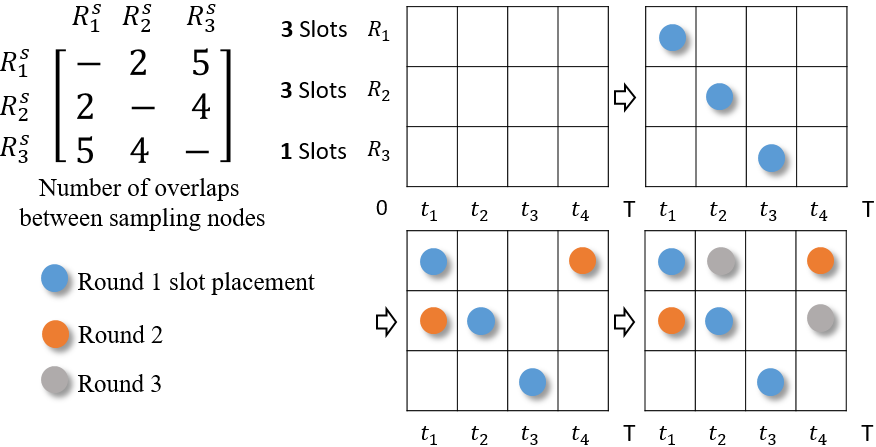
\includegraphics[width=7cm]{images/greedy_for_order_slot.png}
\caption{Illustrating sampling node slots placement based on greedy algorithm}
\label{slot_order}
\end{figure}

\section{Experiments and results}
In order to verify the effectiveness and performance of our algorithm, we have built a laboratory bed based on floodlight controller and openvswitch + mininet. The whole experimental bed contains 12 Dell XPS hosts, 20 core CPU, and Ubuntu 16.06.2 LTS. One runs a floodlight controller that fuses our algorithm, the other runs a data collector, and the remaining 10 deploy a network topology with 110 switch nodes and 50 host nodes. The experimental traffic dataset comes from the open project "the WIDE Project". We selected data from 14:00-14:15 in August 6, 2018. After cleaning and screening, we collate 5000 data streams for experiments. In the experiment, the number of data streams changed from 1000 to 5000..
We implement four algorithms: Random-K, top-K based on the extended median centrality, top-K based on the standard median centrality, our algorithm XXX. Based on the above four algorithms, we have made a comparative experiment in three measurement mechanisms: sampling accuracy, packet repetition rate and the number of rat streams collected.
Fig.x shows the comparison of sampling accuracy in different algorithms. Our algorithm is 7\% higher than Top-k and over 20\% than the other two algorithms. From Fig.x, we can see that different algorithms do almost the same amount of elephant flow collection. In fact, our algorithm only takes more part of the rat flow than other algorithms. And Fig.x shows that our algorithm is effective in reducing duplication and reducing it by more than 30\%.

\begin{figure}[!hhhhhhhhhht]
\centering
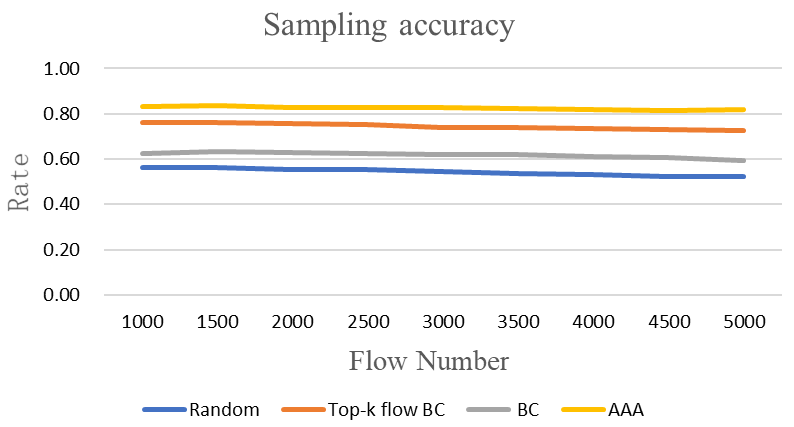
\includegraphics[width=7cm]{images/cmp_sam_accu.png}
\caption{accuracy comparison with respect to different algorithms}
\label{aaa.png}
\end{figure}
\begin{figure}[!hhhhhhhhhht]
\centering
\includegraphics[width=7cm]{images/cmp_rep_rate.png}
\caption{repetition rate comparison with respect to different algorithms}
\label{aaa.png}
\end{figure}

%\begin{figure}[!hhhhhhhhhht]
%\centering
%\includegraphics[width=8cm]{images/cmp_rep_rate.png}
%\caption{repetition rate comparison with respect to different algorithms }
%\label{aaa.png}
%\end{figure}

%\begin{figure}[!!!!!!!!!!!!!!hhhhhhhhhht]
%\centering
%\subfigure[ comparison of sampling accuracy]
%{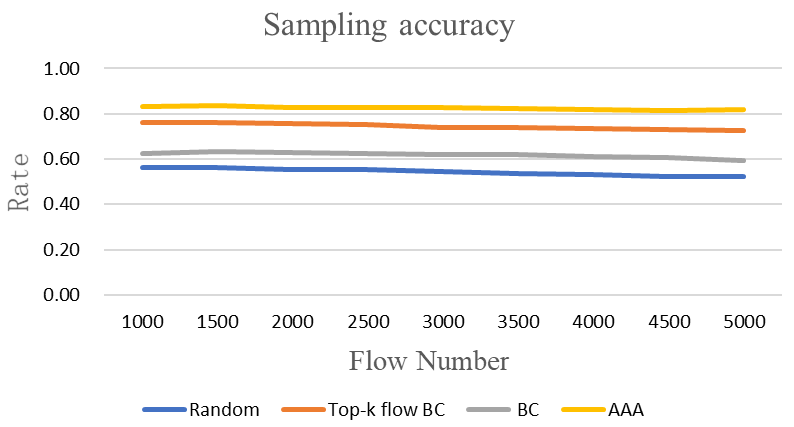
\includegraphics[width=4.1cm]{images/cmp_sam_accu.png}
%\label{fig_x_accu}
%}
%\subfigure[comparison of repetition rate]
%{\includegraphics[width=4.1cm]{images//cmp_rep_rate.png}
%\label{fig_x_rep}
%}
%\caption{comparison with respect to different algorithms}
%\label{fig_x_cmp}
%\end{figure}

\begin{figure}[!hhhhhhhhhht]
\centering
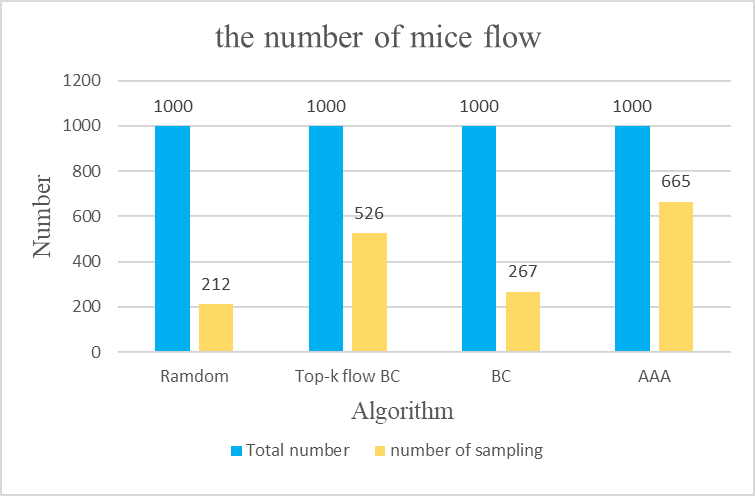
\includegraphics[width=8cm]{images/cmp_mice_flownum.png}
\caption{comparison of different algorithms in number of mice flow}
\label{aaa.png}
\end{figure}

\begin{figure}[!hhhhhhhhhht]
\centering
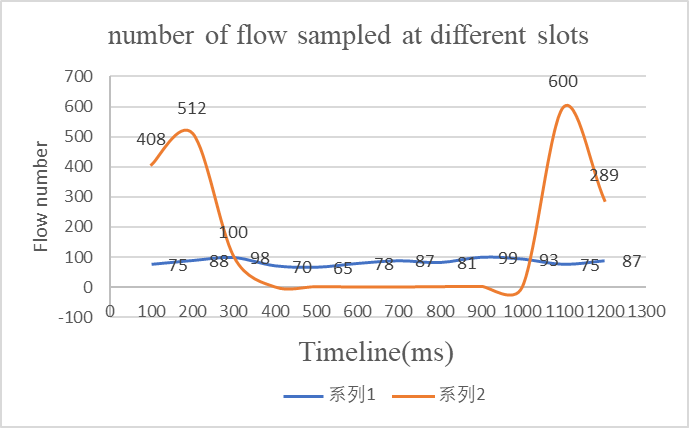
\includegraphics[width=8cm]{images/num_slot.png}
\caption{comparison of sampling flow number at different slot}
\label{aaa.png}
\end{figure}



\section{Conclusion}
\begin{itemize}
\item Lab environment
\item Sampling accuracy comparison
\item Sampling repetition rate comparison
\item Greedy centrality algorithm experimental results
 
\item Deduplication rate algorithm comparison

\item Experimental comparison of adaptive co-sampling algorithm
\end{itemize}



%\section{Conclusion}

%\begin{itemize}
%\item[-] Case 1: $ \frac{1}{SW_{num}} < S_{rate} \Leftrightarrow Confliction $   \\
%\item[-] Case 2: $ \frac{1}{SW_{num}} >= S_{rate} \Leftrightarrow no Confliction $ 


 





% trigger a \newpage just before the given reference
% number - used to balance the columns on the last page
% adjust value as needed - may need to be readjusted if
% the document is modified later
%\IEEEtriggeratref{8}
% The "triggered" command can be changed if desired:
%\IEEEtriggercmd{\enlargethispage{-5in}}

% references section

% can use a bibliography generated by BibTeX as a .bbl file
% BibTeX documentation can be easily obtained at:
% http://mirror.ctan.org/biblio/bibtex/contrib/doc/
% The IEEEtran BibTeX style support page is at:
% http://www.michaelshell.org/tex/ieeetran/bibtex/
%\bibliographystyle{IEEEtran}
% argument is your BibTeX string definitions and bibliography database(s)
%\bibliography{IEEEabrv,../bib/paper}
%
% <OR> manually copy in the resultant .bbl file
% set second argument of \begin to the number of references
% (used to reserve space for the reference number labels box)
\begin{thebibliography}{1}

\bibitem{1}
S.~Yoon, T.~Ha, S.~Kim and H.~Lim,\hskip 1em plus 0.5em minus 0.4em
Scalable Traffic Sampling using Centrality Measure on Software-Defined Networks, in \emph{IEEE Communications Magazine}, pp.43-49, July 2017.

\bibitem{1}
M.~Malboubi, L.~Wang, C.N.~Chuah, P.~Sharma,\hskip 1em plus 0.5em minus 0.4em
Intelligent SDN based Traffic (de)Aggregation and Measurement Paradigm (iSTAMP), in \emph{IEEE INFOCOM}, Apr 2014.

\bibitem{1}
L.~Tong and W.~Gao,\hskip 1em plus 0.5em minus 0.4em
Application-Aware Traffic Scheduling for Workload Offloading in Mobile Clouds, in \emph{IEEE INFOCOM}, pp.1-9, Apr 2016.

\bibitem{1}
J.~Jiang, S.~Ma, B.~Li and B.~Li,\hskip 1em plus 0.5em minus 0.4em
Symbiosis: Network-Aware Task Scheduling in Data-Parallel Frameworks, in \emph{IEEE INFOCOM}, pp.10-14, Apr 2016.

\bibitem{1}
P.~Bakopoulos, K.~Christodoulopoulos, G.~Landi et al,\hskip 1em plus 0.5em minus 0.4em
NEPHELE: An End-to-End Scalable and Dynamically Reconfgurable Optical Architecture for Application-Aware SDN Cloud Data Centers, in \emph{IEEE Communitions Magazine}, pp.178-188, Feb 2018.

\bibitem{2}
J.~Xu, J.Y.~Wang, Q.~Qi, H.F.~Sun and B.~He,\hskip 1em plus 0.5em minus 0.4em
IARA: An Intelligent Application-aware VNF for Network Resource Allocation with Deep Learning, in \emph{IEEE SECON}, pp.1-3, June 2018.

\bibitem{2}
J.~Suh, T.T.~Kwon, C.~Dixon, W.~Felter and J.~Carter,\hskip 1em plus 0.5em minus 0.4em
OpenSample: A Low-latency, Sampling-based Measurement Platform for Commodity SDN, in \emph{IEEE ICDCS}, pp.228-237, July 2014.

\bibitem{2}
Z.~Su, T.~Wang, Y.~Xia and M.~Hamdi,\hskip 1em plus 0.5em minus 0.4em
CeMon: A Cost-effective Flow Monitoring System in Software Defined Networks, in \emph{Computer Networks}, pp.101-115, Dec 2015.

\bibitem{3}
N.F.~Huang, C.C.~Li, C.H.~Li, C.C.~Chen,C.H.~C and I.H.~Hsu,\hskip 1em plus 0.5em minus 0.4em
Application Identification System or SDN QoS based on Machine Learning and DNS Responses, in \emph{APNOMS}, pp.407-410, Sept 2017.

\bibitem{3}
S.~Jeong, D.~Lee, J.~Hyun, J.~Li, and J.W.~Hong,\hskip 1em plus 0.5em minus 0.4em
Application-aware Traffic Engineering in Software-Defined Network, in \emph{APNOMS}, pp.315-318, Sept 2017.

\bibitem{3}
G.~Cheng and Y.~Tang,\hskip 1em plus 0.5em minus 0.4em
eOpenFlow: Software Defined Sampling via a Highly Adoptable OpenFlow Extension, in \emph{IEEE ICC}, pp.1-6, May 2017.


\bibitem{3}
S.~Zhao and D.~Medhi,\hskip 1em plus 0.5em minus 0.4em
Application Performance Optimization Using Application-Aware Networking, in \emph{IEEE NOMS},pp.1-6, Apr 2018.

\bibitem{4}
M.~Malboubi, S.M.~Peng, P.~Sharma and C.N.~Chuah,\hskip 1em plus 0.5em minus 0.4em
A Learning-based Measurement Framework for Traffic Matrix Inference in Software Defined Networks, in \emph{Computers \& Electrical Engineering}, Dec 2017.

\bibitem{4}
K.~Bilal, S.U.~Khan, L.~Zhang et al,\hskip 1em plus 0.5em minus 0.4em
Quantitative comparisons of the state-of-the-art data center architectures, in \emph{Concurrency \& Computation Practice \& Experience}, Dec 2017.

\end{thebibliography}




% that's all folks
\end{document}
